
\oldSection*{Appendix}
\frame[plain]{
    \center \LARGE \bf
    \color{isered} Appendix
}
\setcounter{page}{1}

\begin{frame}
    \frametitle{Google's robots.txt}
    \label{robots}
\begin{figure}[htb]
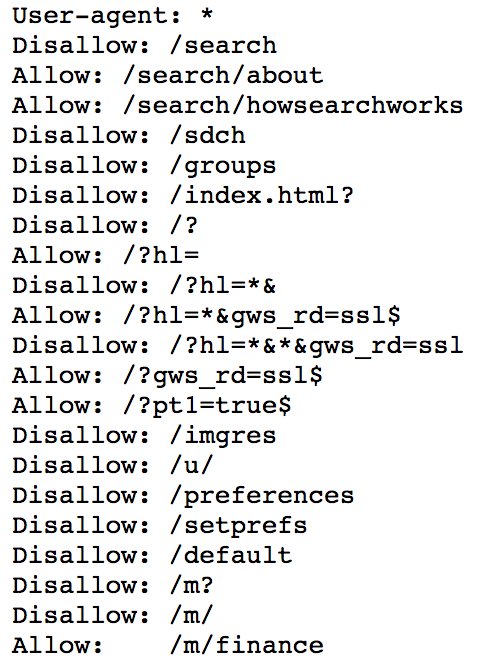
\includegraphics[scale=0.27,left]{img/figures/google_robots}
\end{figure}
\vspace{-40pt}
\begin{flushright}
\hyperlink{manners}{\beamerbutton{Back}}
\end{flushright}
\end{frame}

\begin{frame}
    \label{dependency_tree}
    \frametitle{Grammar based Dependency Tree}
    \begin{figure}[htb]
        \begin{center}
            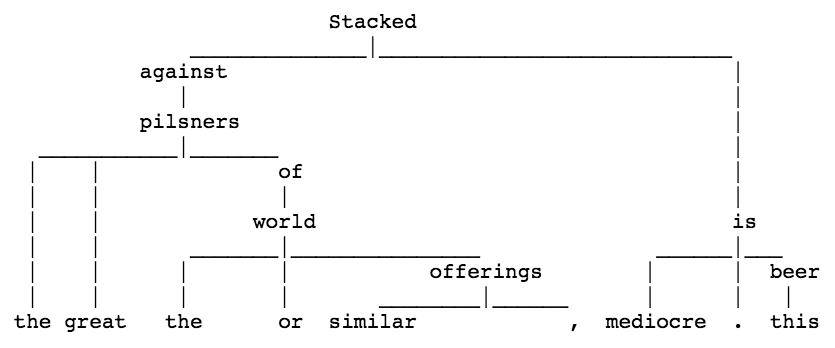
\includegraphics[scale=0.35]{img/figures/dependency_tree}
        \end{center}
    \end{figure}
\begin{flushright}
\hyperlink{review_verbs}{\beamerbutton{Back}}
\end{flushright}
\end{frame}

\begin{frame}
    \frametitle{Summary - All Words}
    \label{text_all}
\begin{figure}[htb]
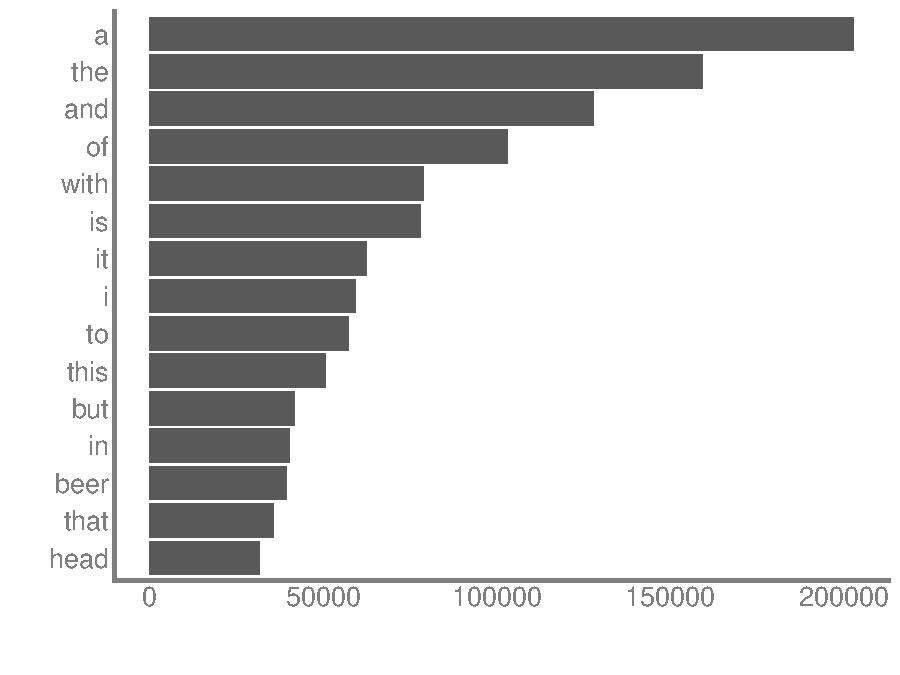
\includegraphics[scale=0.55,left]{img/figures/bar_words}
\end{figure}
\vspace{-40pt}
\begin{flushright}
\hyperlink{beer_review}{\beamerbutton{Back}}
\end{flushright}
\end{frame}


\begin{frame}
    \frametitle{Summary - All Nouns}
    \label{stats_nouns}
\begin{figure}[htb]
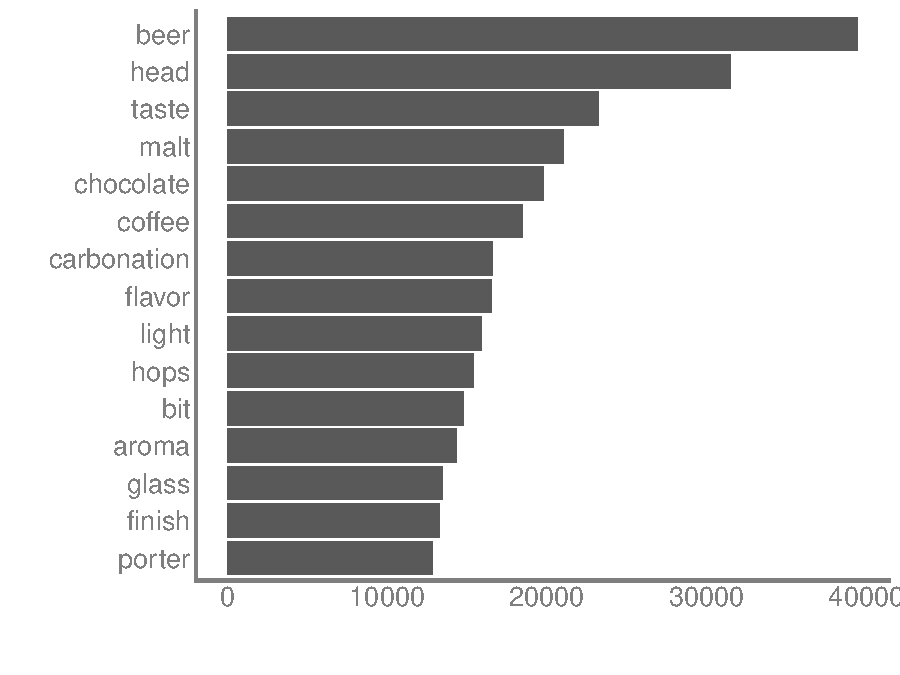
\includegraphics[scale=0.55,left]{img/figures/bar_nouns}
\end{figure}
\vspace{-40pt}
\begin{flushright}
\hyperlink{review_nouns}{\beamerbutton{Back}}
\end{flushright}
\end{frame}

\begin{frame}
    \frametitle{Summary - All Adjectives}
    \label{stats_adjectives}
\begin{figure}[htb]
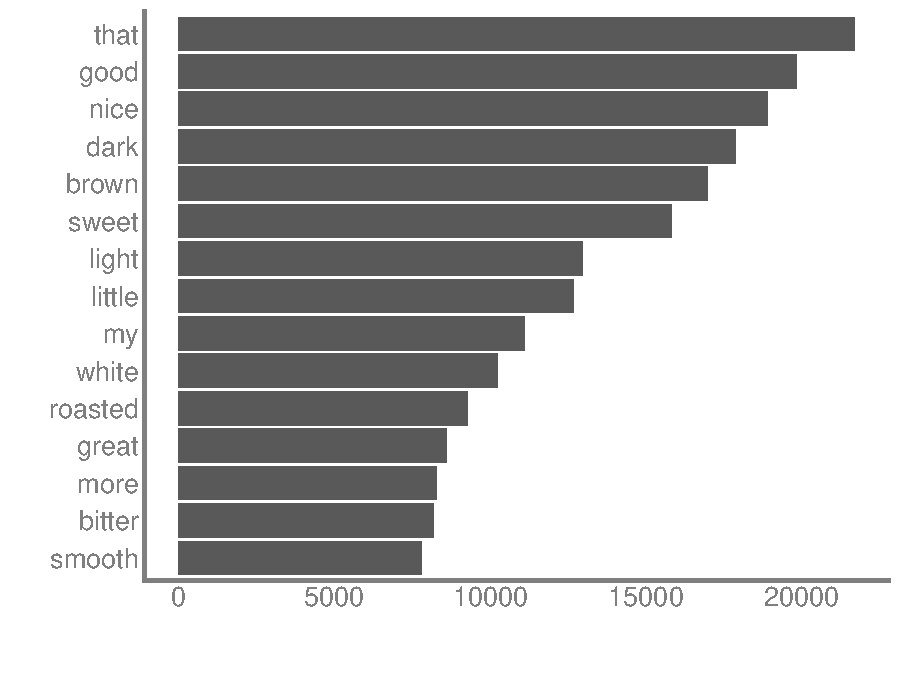
\includegraphics[scale=0.55,left]{img/figures/bar_adj}
\end{figure}
\vspace{-40pt}
\begin{flushright}
\hyperlink{review_adjectives}{\beamerbutton{Back}}
\end{flushright}
\end{frame}